% !TEX root = ../YourName-Dissertation.tex

\chapter{Direct Measurement of the Neutrino Mass with Cyclotron Radiation Emission Spectroscopy}

\section{Introduction}

\section{Cyclotron Radiation Emission Spectroscopy}

Of the standard physical quantities the one that can be measured with the highest precision is time and the inversely related quantity frequency. In fact it is often advantageous to convert measurements of other physical quantities like mass or length into frequency measurements due to the digital nature of frequency measurements that make them immune to many sources of noise. Atomic clocks, which operate by measuring the frequencies of various atomic transitions, have been used to measure time with astounding relative uncertainties of $10^{-18}$~seconds. The extreme precision possible with frequency measurements is often summarized using the a quote from the Physicist Arthur Schawlow who said advise his students to "Never measure anything but frequency!". 

Neutrino mass measurements using tritium beta-decay are effectively attempting to measure  

\begin{figure}[htbp]
    \centering
    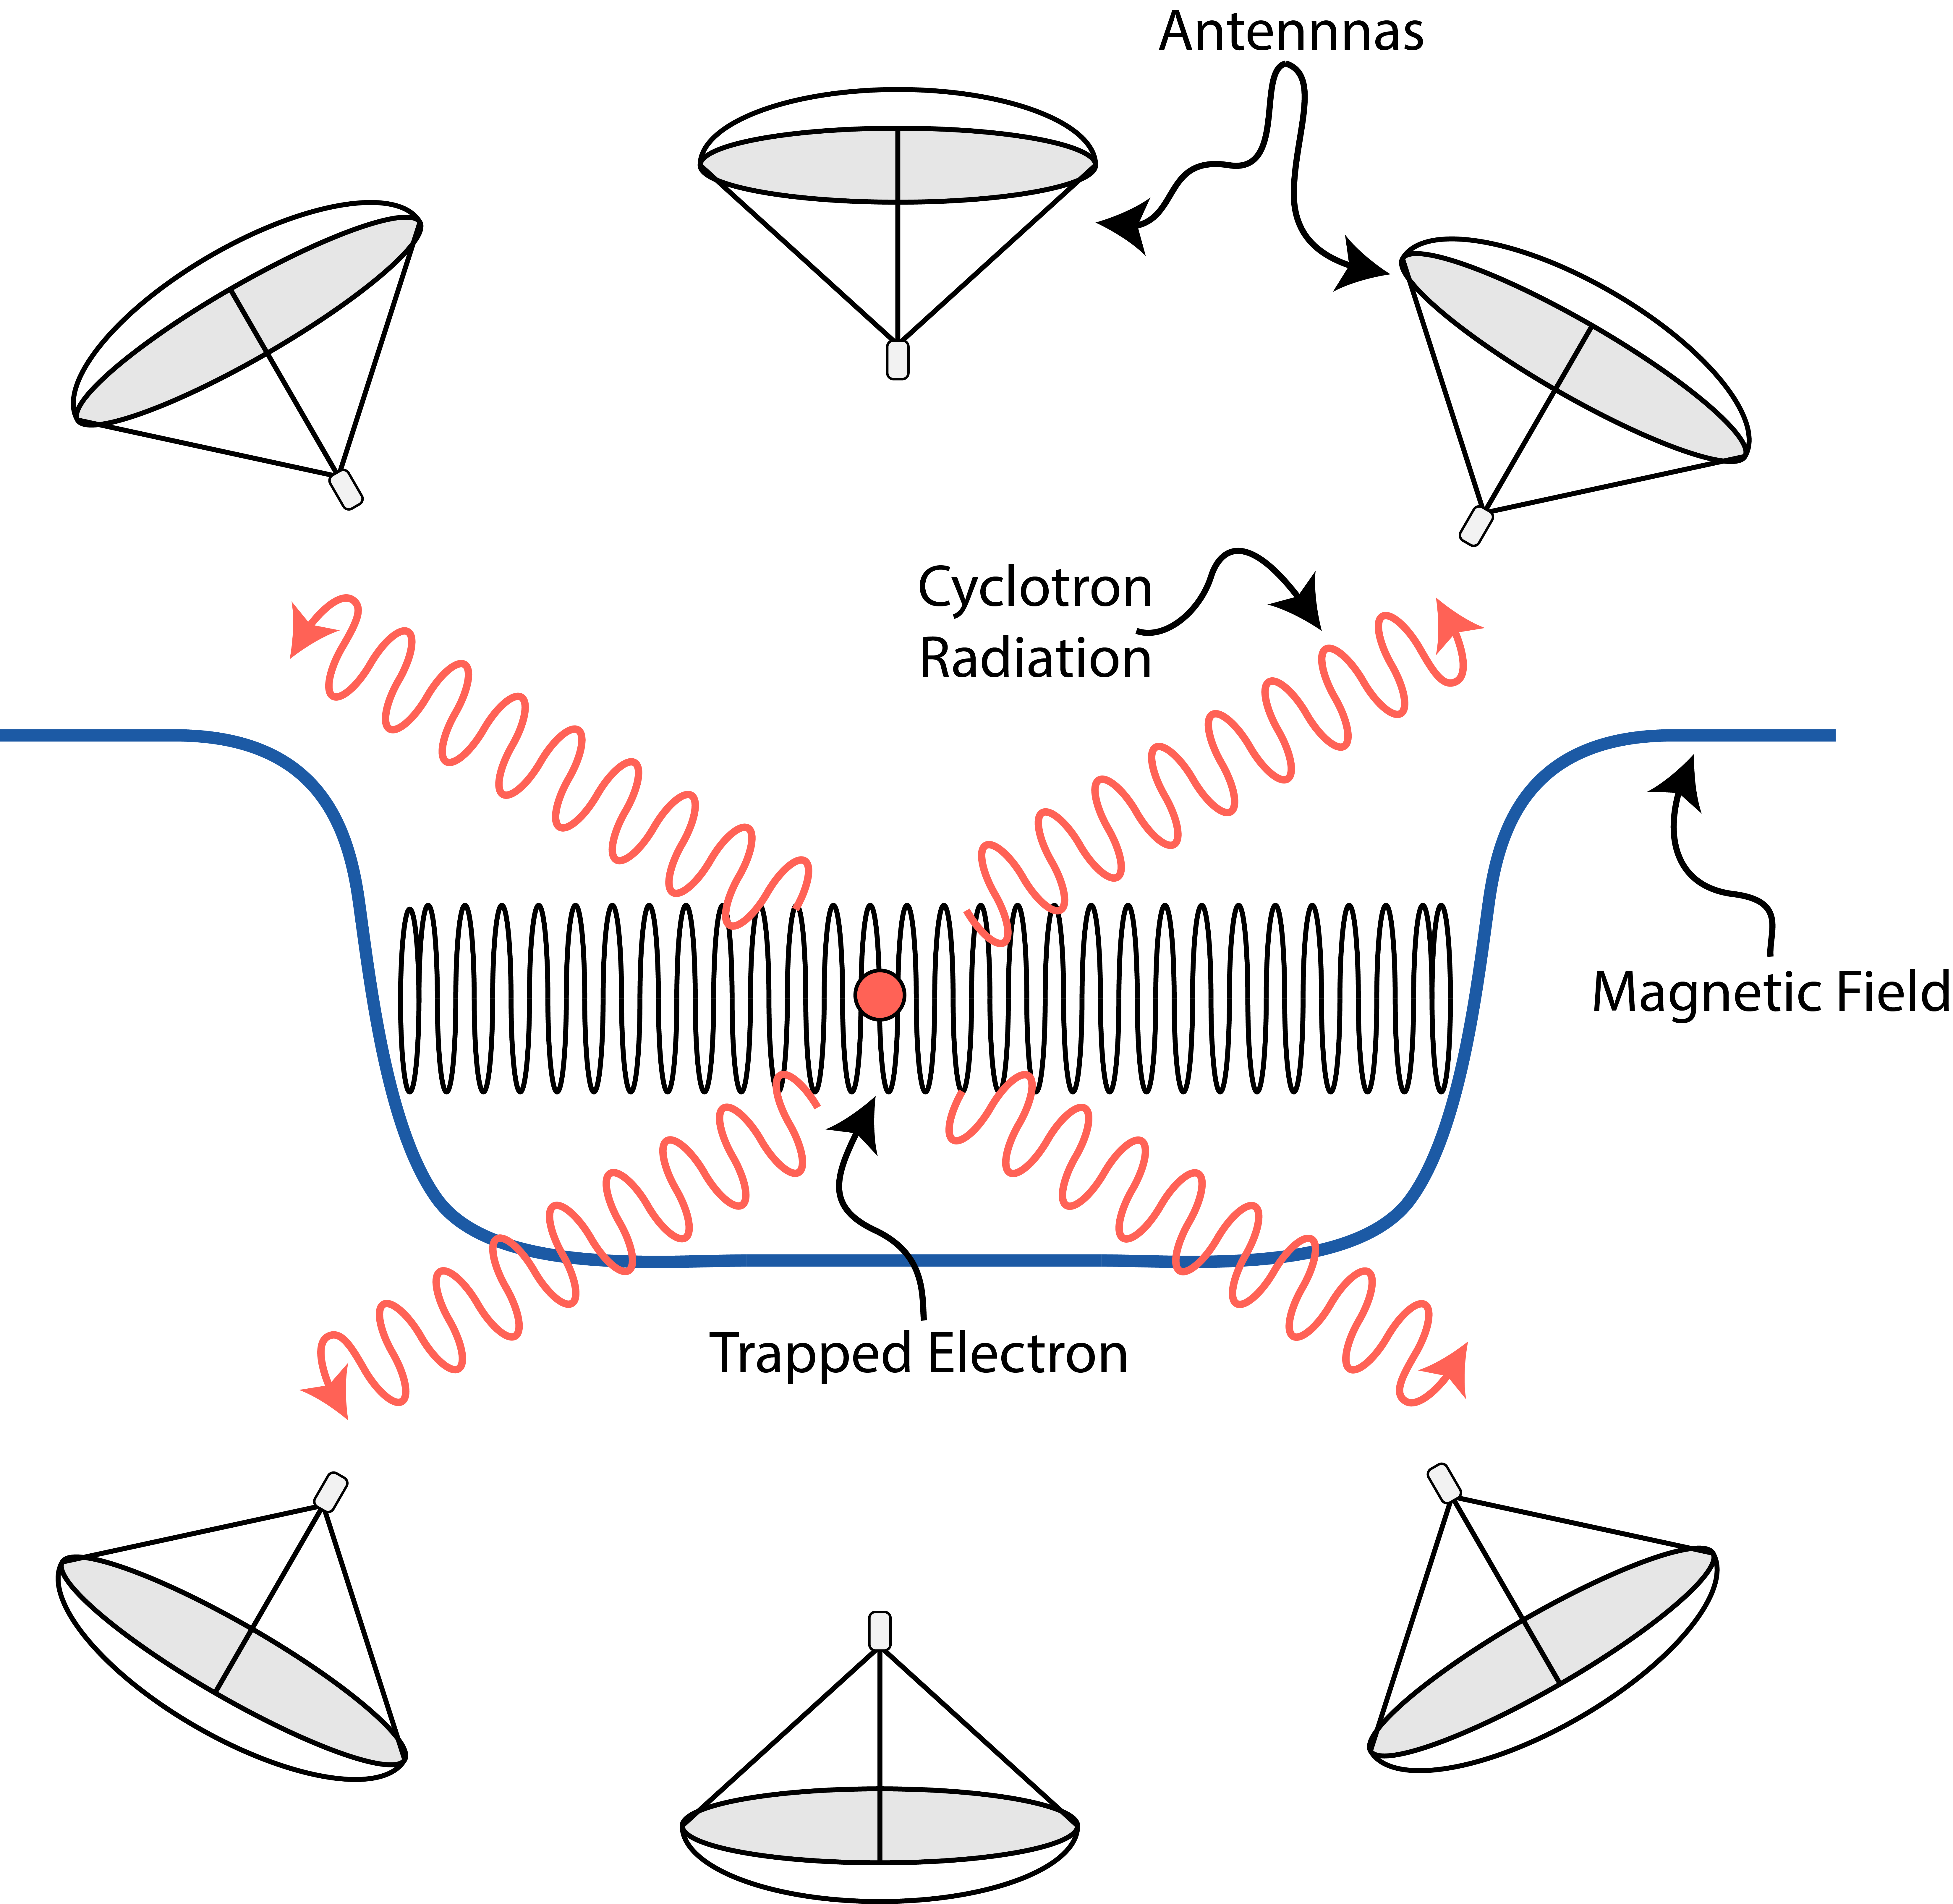
\includegraphics[width=0.5\textwidth]{figs/Chapter-3/230303_cres_cartoon.png}
    \caption{Caption}
    \label{fig:cres_cartoon}
\end{figure}

\subsection{Charged Particles in a Magnetic Trap}

\begin{figure}[htbp]
    \centering
    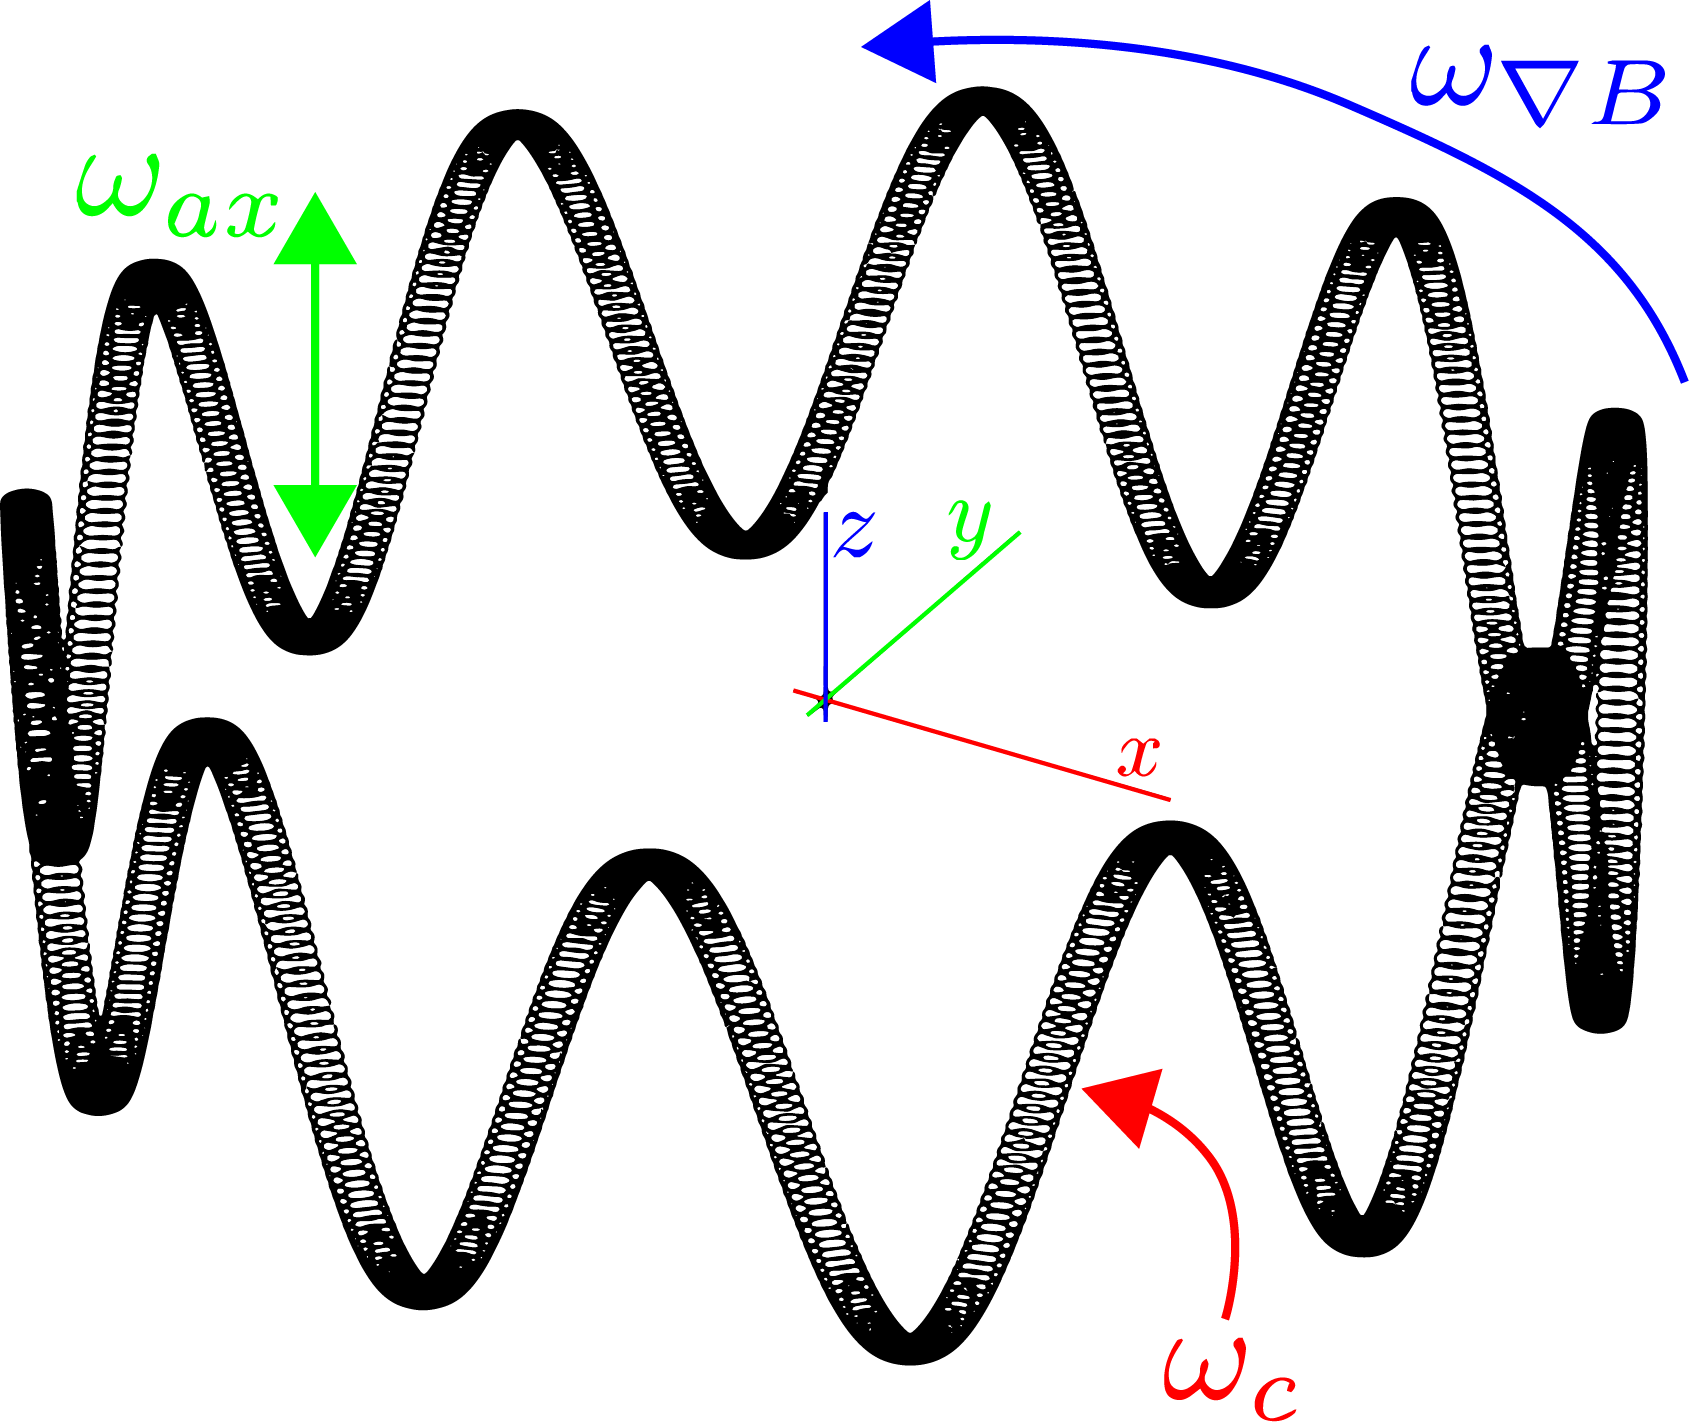
\includegraphics[width=0.5\textwidth]{figs/Chapter-3/230511_trapped_motion.png}
    \caption{Caption}
    \label{fig:chap3-trapped-electron-motion}
\end{figure}

\subsection{Radiation from a Charged Particle}

\section{The Project 8 Collaboration}

\subsection{Neutrino Mass Sensitivity Goals}

\subsection{Phased Development Plans}

\begin{figure}[htbp]
    \centering
    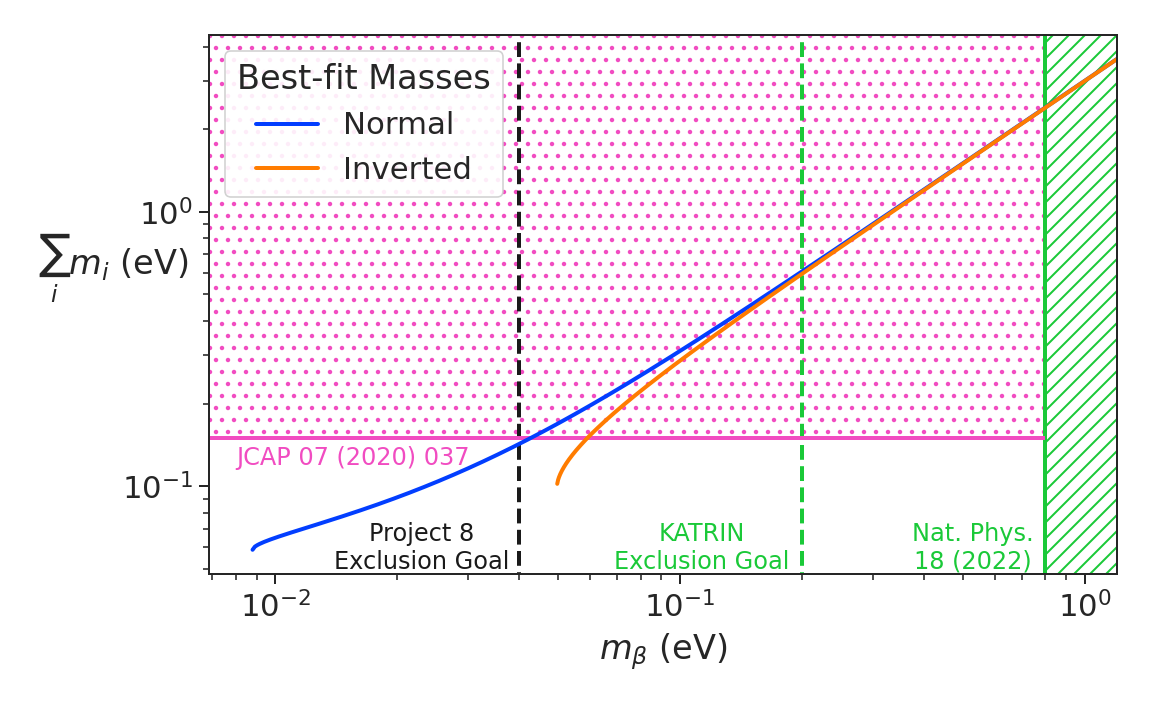
\includegraphics[width=0.7\textwidth]{figs/Chapter-3/230303_sum_nu_mass_vs_m_beta_with_exclusion_and_goal.png}
    \caption{Caption}
    \label{fig:p8_nu_mass_goal}
\end{figure}

\section{Phase II: First Tritium Beta Decay Spectrum and Neutrino Mass Measurement with CRES}

\subsection{The Project 8 CRES Demonstrator}

\begin{figure}[htbp]
    \centering
    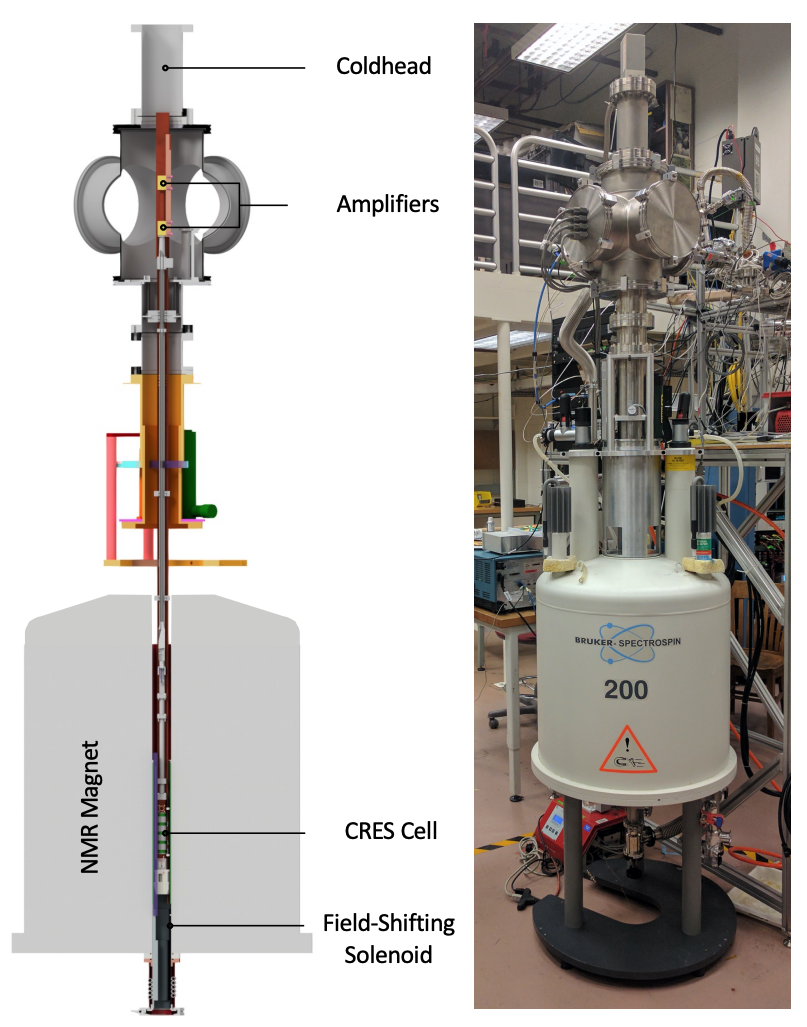
\includegraphics[width=0.7\textwidth]{figs/Chapter-3/phaseII_system.png}
    \caption{Caption}
    \label{fig:phase2_apparatus}
\end{figure}

\begin{figure}[htbp]
    \centering
    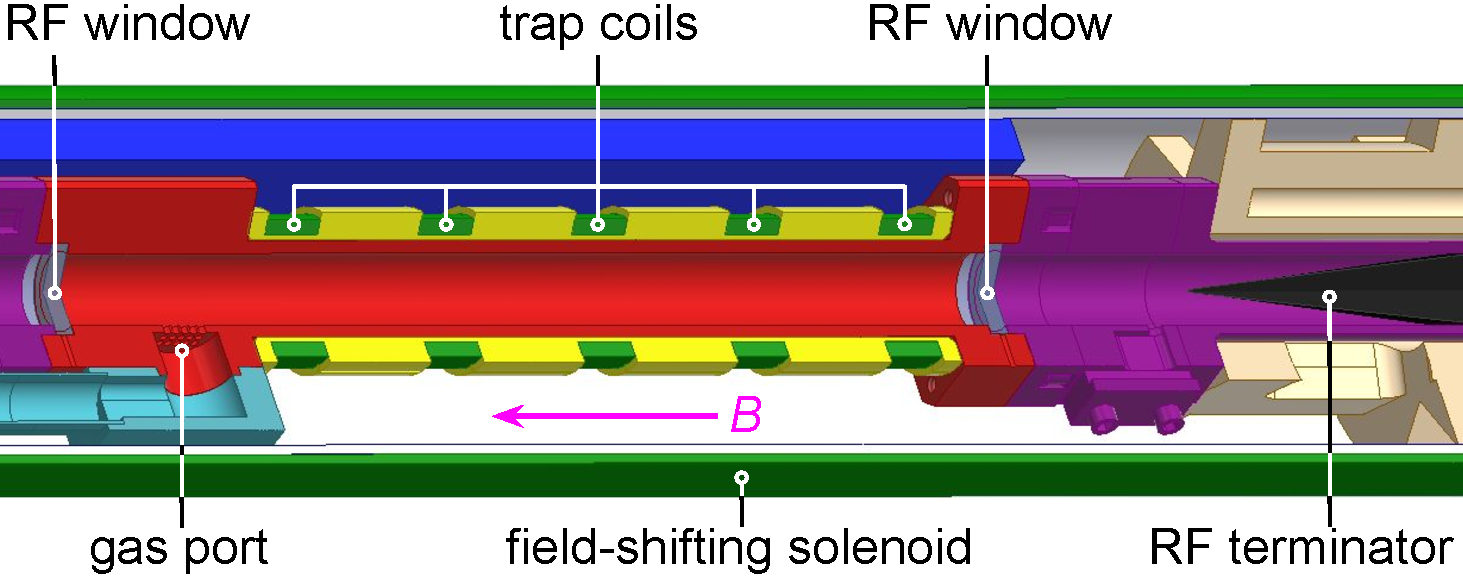
\includegraphics[width=0.8\textwidth]{figs/Chapter-3/apparatus.pdf}
    \caption{Caption}
    \label{fig:phase2_cres_cell}
\end{figure}

\subsection{CRES Track and Event Reconstruction}

\begin{figure}[htbp]
    \centering
    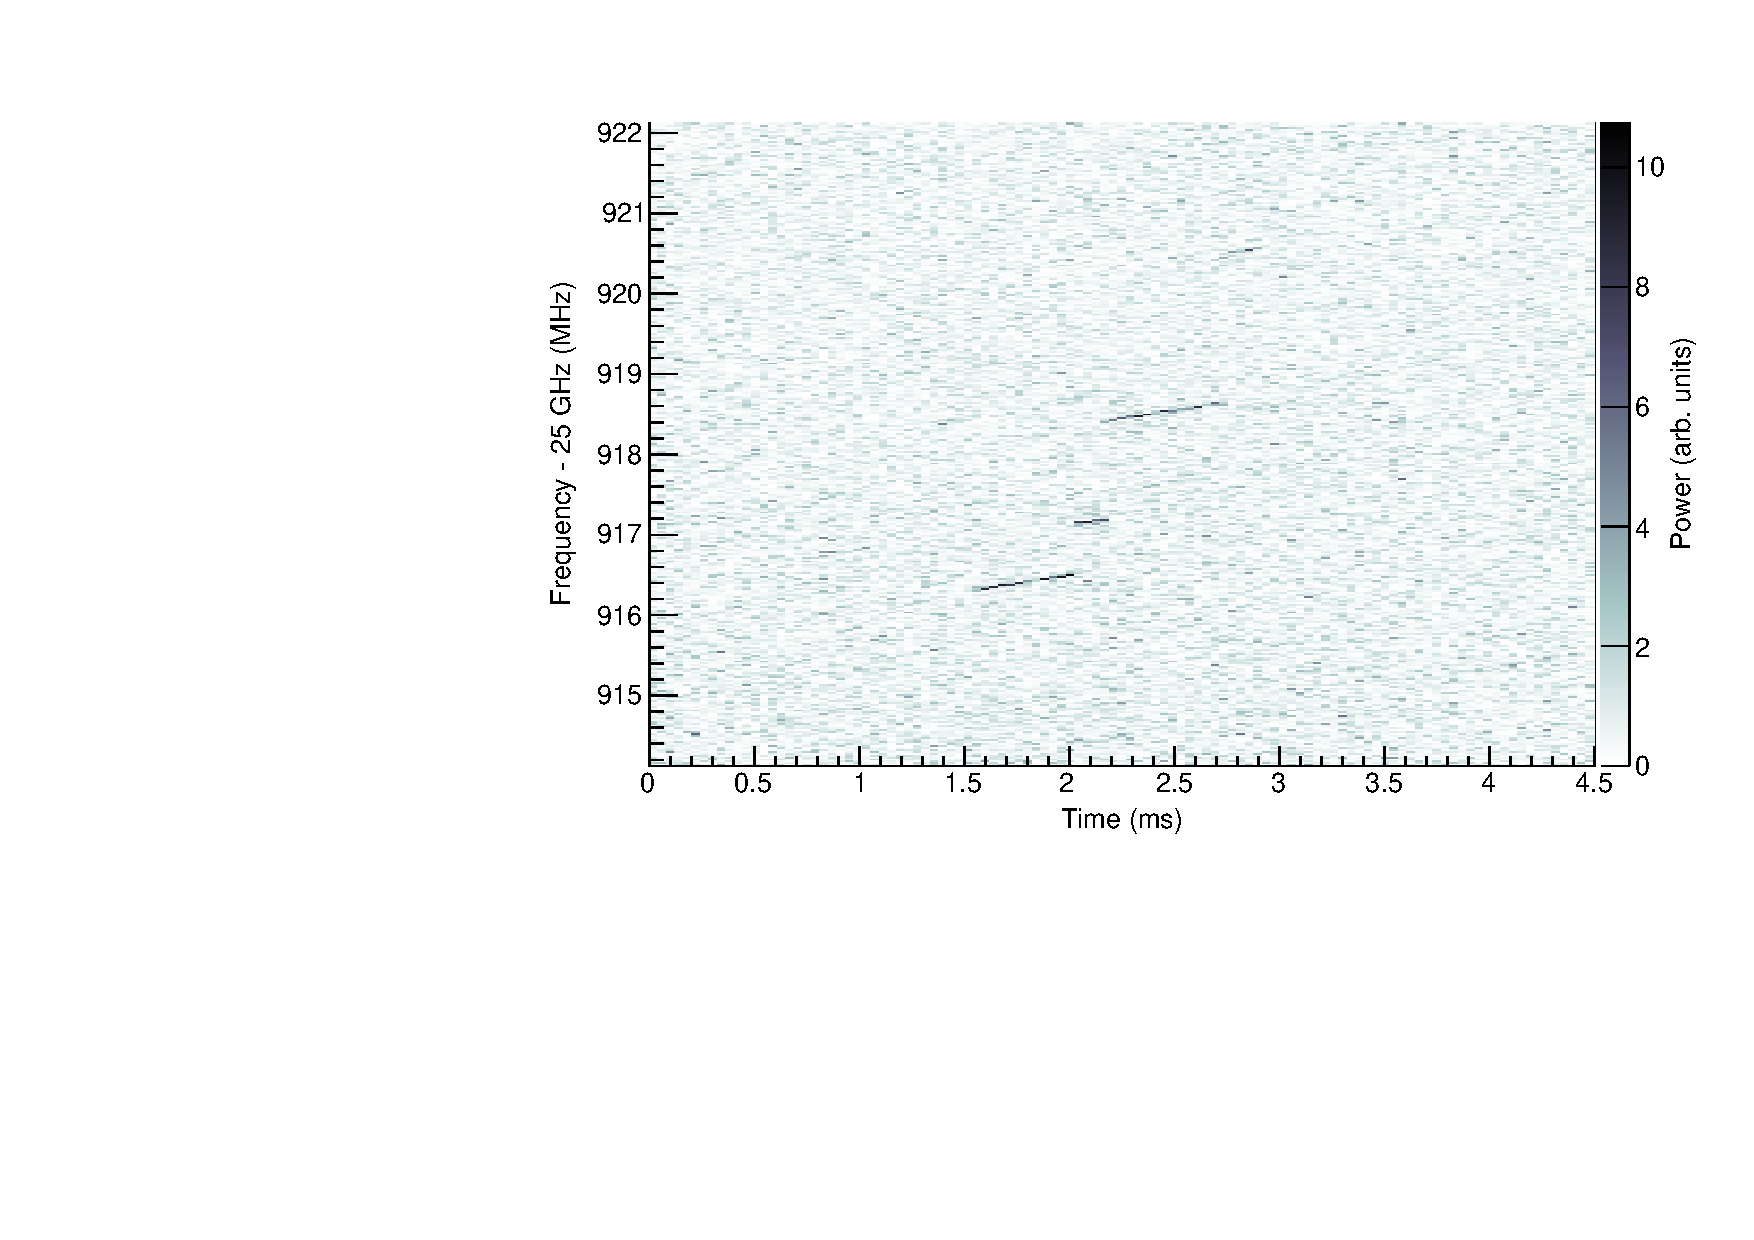
\includegraphics[width=0.7\textwidth]{figs/Chapter-3/T2_Event0.pdf}
    \caption{Caption}
    \label{fig:tritium_event0}
\end{figure}

\subsection{Measurements with Krypton}

\begin{figure}[htbp]
    \centering
    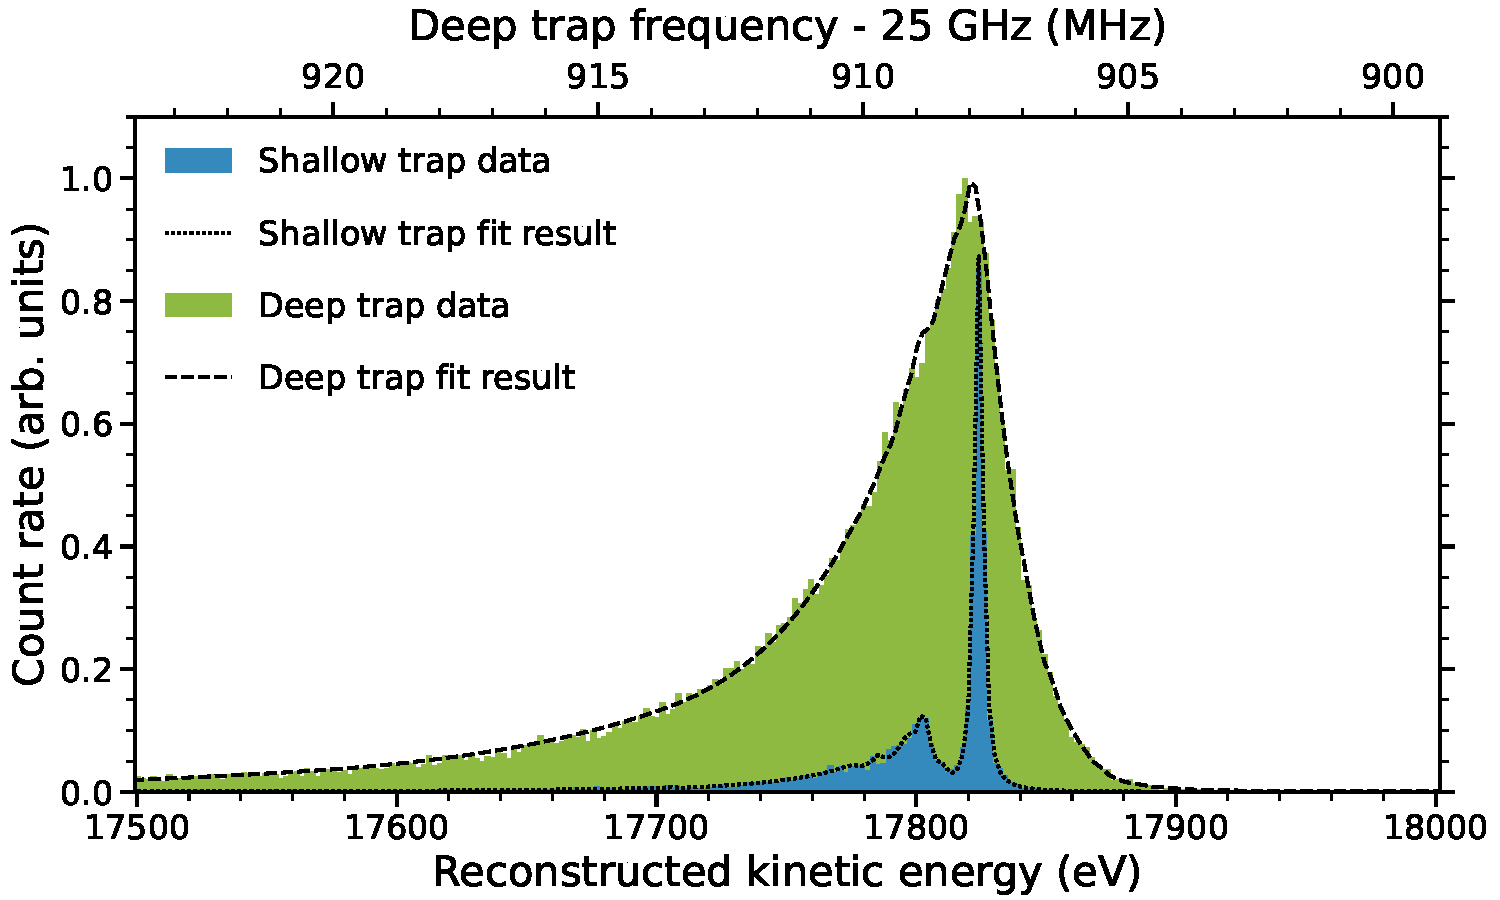
\includegraphics[width=0.7\textwidth]{figs/Chapter-3/kr_fit.pdf}
    \caption{Caption}
    \label{fig:krypton_fit}
\end{figure}

\begin{figure}[htbp]
    \centering
    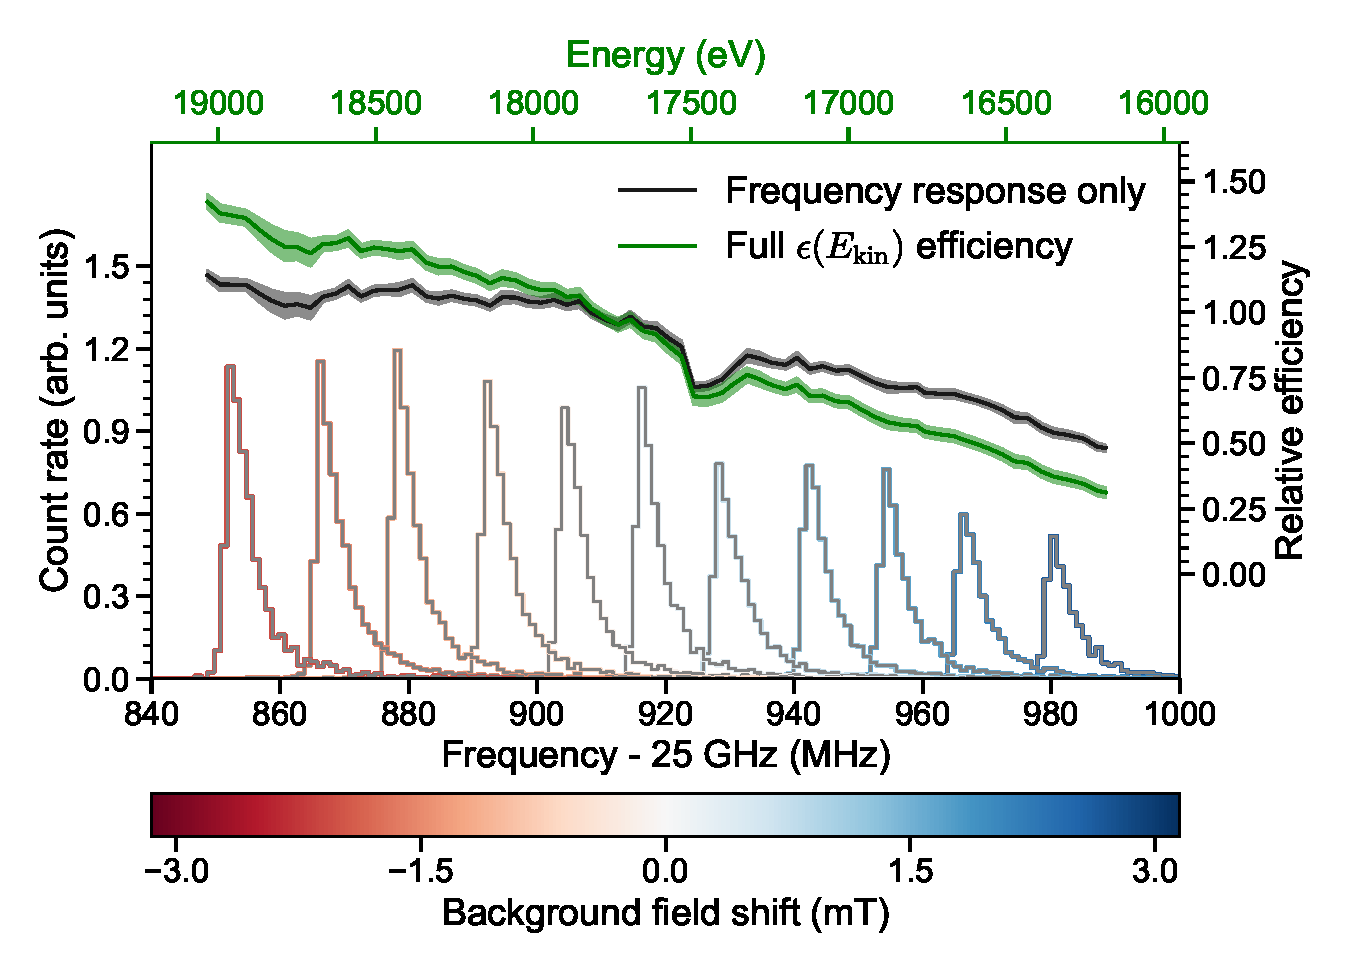
\includegraphics[width=0.7\textwidth]{figs/Chapter-3/fss_for_prl_plot.pdf}
    \caption{Caption}
    \label{fig:fss_plot}
\end{figure}

\subsection{Tritium Spectrum and Neutrino Mass Results}

\begin{figure}
    \centering
    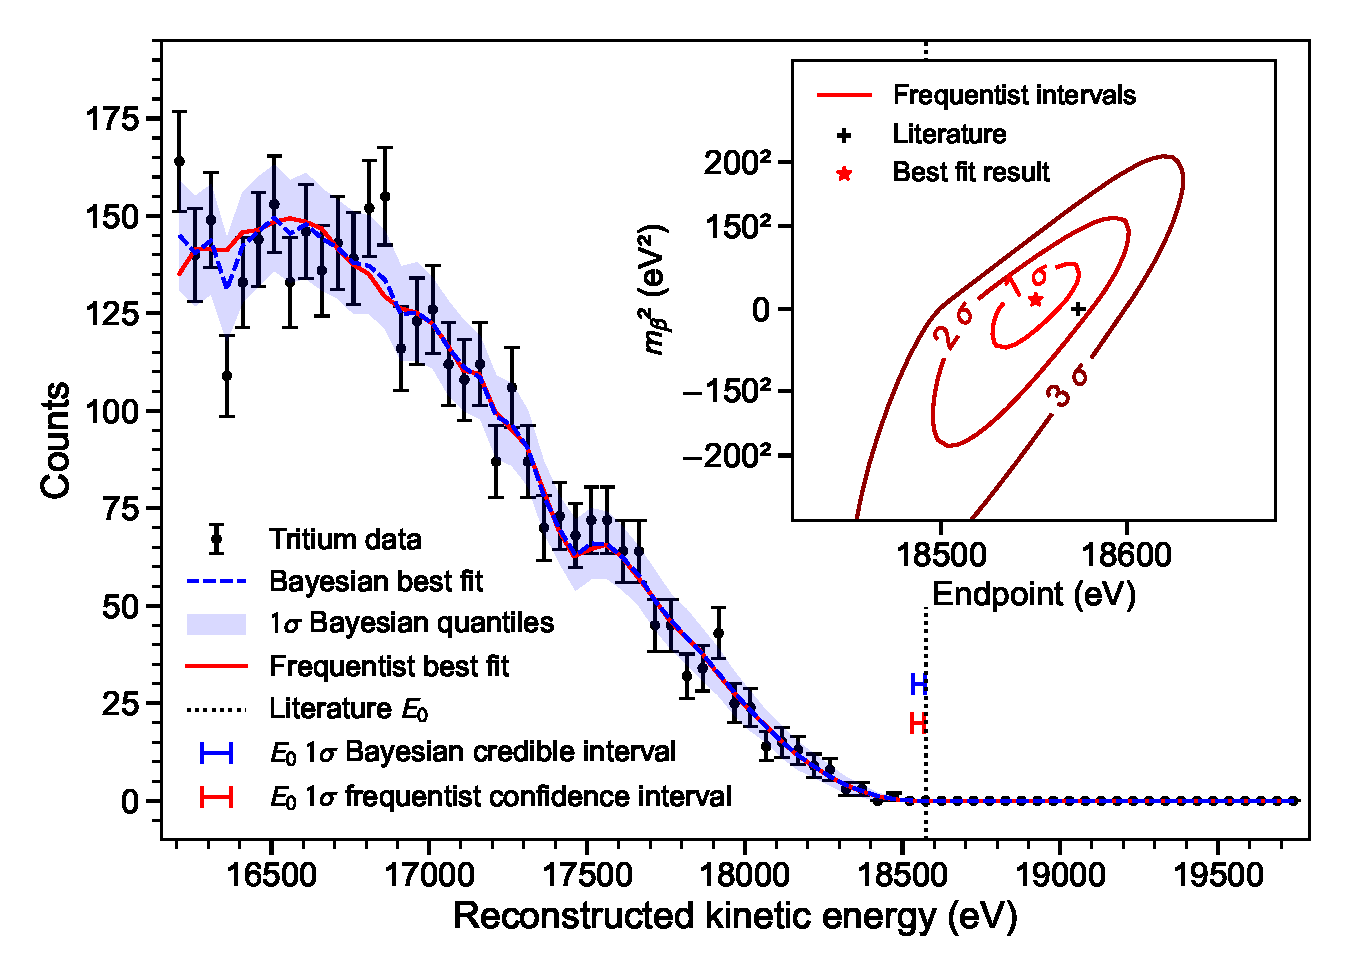
\includegraphics[width=0.7\textwidth]{figs/Chapter-3/12-03-22A_final_E0_real_data_phase_II_tritium_fit_1d.pdf}
    \caption{Caption}
    \label{fig:final_tritium_fit}
\end{figure}

\section{Phase III: Developing Free-space CRES Measurements with Antenna Arrays}

The goal of Phase III in the Project 8 experimental program is to develop the technologies and expertise required to build an experiment that uses CRES to measure the neutrino mass with a target sensitivity of 40~meV. One of the key technologies is a method for performing high resolution CRES measurements in a large volume, which allows one to observe a sufficient quantity of tritium to measure the low-activity endpoint region of the tritium spectrum. 

\subsection{The Basic Approach}

One possible approach, suggested in the original CRES publication, is to use many antennas to surround a volume of tritium gas in a magnetic field (see Figure \ref{fig:chap3-antenna-concept-cartoon}). When a decay occurs the electron will begin to emit cyclotron radiation that can be collected by the array and used to perform CRES.
\begin{figure}[htbp]
    \centering
    \includegraphics*[width=0.6\textwidth]{figs/Chapter-3/230614_antenna_cartoon.png}
    \caption{\label{fig:chap3-antenna-concept-cartoon}}
\end{figure}
Each antenna in the array collects only a small fraction of the electron's signal power, which is less than 1~fW for a 18.6~keV kinetic energy electron in a 1~T magnetic field. Scaling to large volumes with the antenna array approach is accomplished by increasing the number of antennas in the array, which increases the volume under observation proportionally, so that a sufficient population of tritium atoms can be observed to measure the tritium spectrum endpoint shape. 

Several features of the antenna array approach make it an attractive candidate technology for a large volume experiment. One example is the accurate position reconstruction made possible by the multichannel nature of the array. Using techniques like digital beamforming it is possible to estimate the radial and azimuthal positions of the electron in the magnetic trap with a precision significantly less than the size of the cyclotron wavelength. This capability allows one to perform event-by-event estimations of the magnetic field experienced by an electron, which is crucial to achieving high energy resolution with the CRES technique.

The easy availability of position information with the antennas array approach is potentially a unique advantage that provides significant flexibility in the magnetic field uniformity requirements compared to other proposed approaches to large volume CRES (see Chapter \ref{chap:cavity}). Spatial discrimination using digital beamforming leads to pileup reduction, which helps to reduce the potential of background events caused by missing tracks or by incorrectly clustering a group of tracks into an event. Limits on the background rate for a neutrino mass measurement with 40~meV sensitivity are stringent and the total activity of the tritium source for such an experiment is gigantic relative to the activity near the endpoint. Thus, pileup discrimination could be an important tool for a large scale CRES experiment.

Another beneficial quality of the antenna array approach is that the volume of the experiment can be scaled independent of frequency by simply adding more antennas to the array. Resonant cavities, the proposed alternative large volume CRES technology, are ideally operated in magnetic fields that cause electrons to move with cyclotron frequencies near the fundamental cavity resonance, to avoid complex coupling of the electron to many cavity modes simultaneously. This leads to a coupling between the cavity volume and the magnetic field magnitude, which forces one to lower the magnetic field in order to increase the experiment scale. Whereas, for antenna arrays, in principle there is no physical limitation on the size of the antenna array that can be used at a particular magnetic field. However, the nature of scaling an antenna array based experiment leads to rapidly increasing cost and complexity due to the large number of antennas, amplifiers, and data streams that require substantial computer processing power to effectively analyze.

\subsection{The FSCD: Free-space CRES Demonstrator}

The complex collection of new experimental techniques and methods that come together in the antenna array CRES technique require the construction of a small scale demonstration experiment designed to develop an understanding of the principles of antenna array CRES measurements and the relevant systematics. Without operating such an experiment it is not possible to develop a design for a large scale CRES experiment with sufficient confidence that the experiment is capable of measuring the shape of the tritium spectrum endpoint to the degree of accuracy required for 40~meV sensitivity to the neutrino mass. Therefore, Phase III of the Project 8 experimental program is primarily focused on the development and operation of demonstrator experiments to inform the design of the final Phase IV experiment.

Specifically for antenna array CRES, the associated demonstrator experiment in Phase III is called the Free-space CRES Demonstrator or FSCD. The goals of the FSCD include not only the development of antenna array CRES itself, but is also a capable neutrino mass measurement experiment in it's own right, with a target neutrino mass sensitivity of a few eV using a molecular tritium source.  

\subsubsection*{Magnetic Field}

The background magnetic field for the FSCD experiment is provided by a hospital-grade MRI magnet (see Figure \ref{fig:chap3-mri-magnet}). The magnet produces a magnetic field of approximately 0.958~T, which corresponds to a tritium spectrum endpoint frequency of approximately 25.86~GHz. 
\begin{figure}[htbp]
    \centering
    \includegraphics*[width=0.5\textwidth]{figs/Chapter-3/230614_mri_magnet.png}
    \caption{\label{fig:chap3-mri-magnet}}
\end{figure}
The magnet is installed in the Project 8 laboratory located at the University of Washington, Seattle, and is shimmed to produce a uniform magnetic field with variations on the ppm scale. Measurements of the magnetic field non-uniformities were performed using a NMR probe and rotational gantry to capture measurements of the magnetic field around an elliptical surface in the center of the MRI magnet. During the operation of the FSCD an array of Hall or NMR magnetometers could be used to periodical measure the magnetic field in order to quantify its time stability.

Inside the main magnetic field of the MRI magnet are additional magnets that provide the capability to shift the value of the background magnetic field as well as the magnets that produce the magnetic trap. Shifting the background value of the magnetic field on a scale of $O(\mu T)$ allows one to control the cyclotron frequencies of electrons with a fixed kinetic energy, which is key to effectively calibrating the FSCD. The preferred calibration method for the FSCD is a mono-energetic electron gun that can inject electrons into the magnetic trap with a known kinetic energy. In combination with the field shifting magnet one can vary the cyclotron frequencies of the electrons to measure the response of the antenna array as a function of the radiation frequency and electron position. This procedure not only characterizes the response of the antenna array but also provides further information on magnetic field uniformity, which important to achieving optimal energy resolution.

Several additional magnetic coils will need to included inside the MRI magnet to produce the magnetic trap. The ideal trap shape for CRES is the perfect magnetic box, which has a flat bottom and step function walls. Any variation in the average magnetic field experienced by an electron leads to changes in the cyclotron frequency that can make determining the true starting kinetic energy more difficult. This includes changes in the magnetic field caused by the walls of the magnetic trap as well as radial magnetic field variations. The perfect box trap is completely uniform and has infinitely steep walls that cause no change in the electron's cyclotron frequency as it is reflected from the trap wall, however, such a trap cannot be made from any combination of magnetic coils since it violates Maxwell's equations. The goal of magnetic trap design is to identify the configuration of coils that produces a trap that approximates the perfect box trap as closely as possible.

\subsubsection*{Antenna Array}

The canonical antenna array design for a CRES experiment is a uniform cylindrical array of antennas that surrounds the magnetic trap volume. Since the FSCD is a demonstrator experiment, the antenna array design is the simplest form of the uniform cylindrical array, which is a single circular ring of antennas with a diameter of 20~cm (see Figure \ref{fig:chap3-fscd-render}).
\begin{figure}[htbp]
    \centering
    \begin{subfigure}{0.7\textwidth}
        \includegraphics*[width=\textwidth]{figs/Chapter-3/230614_fscd_render.png}
        \caption{}
    \end{subfigure}
    \hfill
    \begin{subfigure}{0.4\textwidth}
        \includegraphics*[width=\textwidth]{figs/Chapter-3/230614_5slot_model.png}
        \caption{}
    \end{subfigure}
    \caption{\label{fig:chap3-fscd-render} (a) A model of the FSCD antenna array, magnetic trap, and tritium containment vessel design.(b) A more detailed model of a prototype design for the 5-slot waveguide antenna design.}
\end{figure}
Along this circle are sixty slotted waveguide antennas that fully populate the available space around the array circumference. In order to maximize the power collected from each electron it is optimal to cover as large a fraction of the solid angle around the magnetic trap as possible. 

The distance between antennas around the circumference of the array is proportional to the wavelength of the cyclotron radiation. Therefore, maximizing the solid angle coverage of the array, while minimizing channel count to keep the hardware and data acquisition costs manageable, biases one towards smaller array diameters. Antenna near-field effects limit the minimum diameter of the array for a given antenna design since the radiation from electron's that are too close to the array cannot be detected due to destructive interference caused by path-length differences from the electron to different points on the antenna surface. 

Slotted waveguide antennas are used in the FSCD antenna array due to their high efficiency and low loss, which comes from the lack of dielectric materials in the antenna structure. Coupling to the waveguide can be performed with a coaxial cable connected at the center or on either end of the waveguide. One of the drawbacks of waveguide antennas is the large amount of space required to fit them inside the limited MRI magnet volume. Alternative antenna designs, constructed from microstrip printed circuit boards require significantly less space at the cost of slightly higher energy loss in the antenna structure. 

The FSCD antenna design is a 5~cm long segment of WR-34 waveguide with 5 vertical slots cut into the side. The distance between slots along the length of the waveguide is a half wavelength for optimal power combination between the individual antenna slots. Each slot is offset from the center of the antenna face a small distance in order to most effectively couple the slot to waveguide modes inside the antenna.

The passive power combination achieved by placing 5 slots in a single waveguide is a compromise intended to reduce the cost and complexity of the antenna array system. Each additional channel in the array requires it's own cryogenic amplifier and also increase the required computer power to process the raw data collected by digitizing each channel. Passive summation, achieved by combining antennas into arrays axially, reduces the array channel count at the cost of losses from imperfect passive combination. Imperfect passive combination is caused by effects such as re-radiation of energy from and destructive interference between slots in the waveguide antenna.






\subsubsection*{Gas System and Tritium Source}

\subsubsection*{Data Acquisition and Reconstruction}

\subsubsection*{Neutrino Mass Sensitivity}

\subsubsection*{Scaling}

\begin{figure}[htbp]
    \centering
    \includegraphics*[width=1\textwidth]{figs/Chapter-3/phaseiv_concept_sketch_ver2.png}
    \caption{}
\end{figure}


